\chapter{Einführung}
\label{chapter:Einfuhrung}
\section{Motivation}
Die Welt wächst zusammen, die Kommunikation steigt und mit ihr auch das Datenvolumen. Waren es 2005 geschätzte 130 Exabyte (130 Mrd. GB) an erzeugten Daten weltweit, so hat sich die Menge bis 2012 um das 20-fache auf 2837 Exabyte gesteigert und 2015 soll die Marke der Zettabyte gebrochen werden, ganze 40000 Exabyte werden an Daten erwartet, die Menge verdoppelt sich jährlich \cite{statista}.\\
%Der Begriff Big Data ist weit gefasst, verstehen die meisten darunter den Rohstoff zur Analyse digitaler Profile von Menschen, so sind ihr Kern doch Daten, denn das Potential der Digitalisierung steigt ins Unermessliche.
%Daten werden maschinell generiert, allein mit RFID-Chips werden Tiere gebrandmarkt, Menschen geben ihre Arbeitszeiten durch, selbst Mülltonen werden damit gekennzeichnet. Neue Technologie ergibt bessere Sensoren mit automatisierteren Abläufen, damit nützt sie vor allem der Forschung: noch mehr Ergebnisse, noch genauere Vorhersagen machen noch präziseres Reagieren in Klimaforschung, Geologie und Physik möglich.\\
Für den Austausch benötigt man die Daten und damit ein geeignetes Datenformat, eines hat sich schlichtweg durchgesetzt: die CSV-Datei - ein portables und menschenlesbares Format zur Darstellung tabellen-ähnlicher Daten.
Aber zur Analyse allein reicht ein Datenformat nicht aus, es müssen Abfragen darüber laufen, die einem Zugriff verschaffen. Die Lösung sind ganz klar relationale Datenbanken mit einer eigenen Abfragesprache, dennoch scheint unter Wissenschaftlern und Firmen eine Ablehnung gegenüber proprietären Datenbanksystemen zu herrschen, da sie ihre Daten lieber in Textform und CSV-Dateien halten.\\
Schaut man in einem Standardwerk zur Datenhaltung für Geowissenschaftler nach, so schlägt es gleichrangig zwei Konzepte vor: textbasierte Datenbanken (wie CSV-Dateien) und relationale Datenbanken. Der anschließende Vergleich erkennt: textbasierte Datenbanken benötigen zum Zugriff "`ein Skript, dass die Datei öffnet und in der ganzen Datei sucht"' \cite[S. 19]{Geo}.
Diese Skripte sind auf unixoiden Systemen meist Bash-Skripte die schwierig zu schreiben, zu warten und in der Ausführung sehr langsam sind.\\
Doch zurück zu großen Datenmengen, was passiert wenn die Daten zu groß werden? Die Abfragezeit mit Skripten explodiert. Will man ein Datenbanksystem zu Hilfe ziehen, so unterstützen sie CSV-Dateien nur unzureichend, sie müssen zuerst geladen werden oder, wie es Oracle anbietet, als \textit{external table} in die Datenbank eingebunden, beides ist teuer.
Programme, die für den CSV-Import in Datenbanken sorgen, gibt es genügend.
Darum stellt diese Arbeit ein Verfahren vor, wie Skripte in SQL-Abfragen umgewandelt werden.
\begin{figure}
\centering
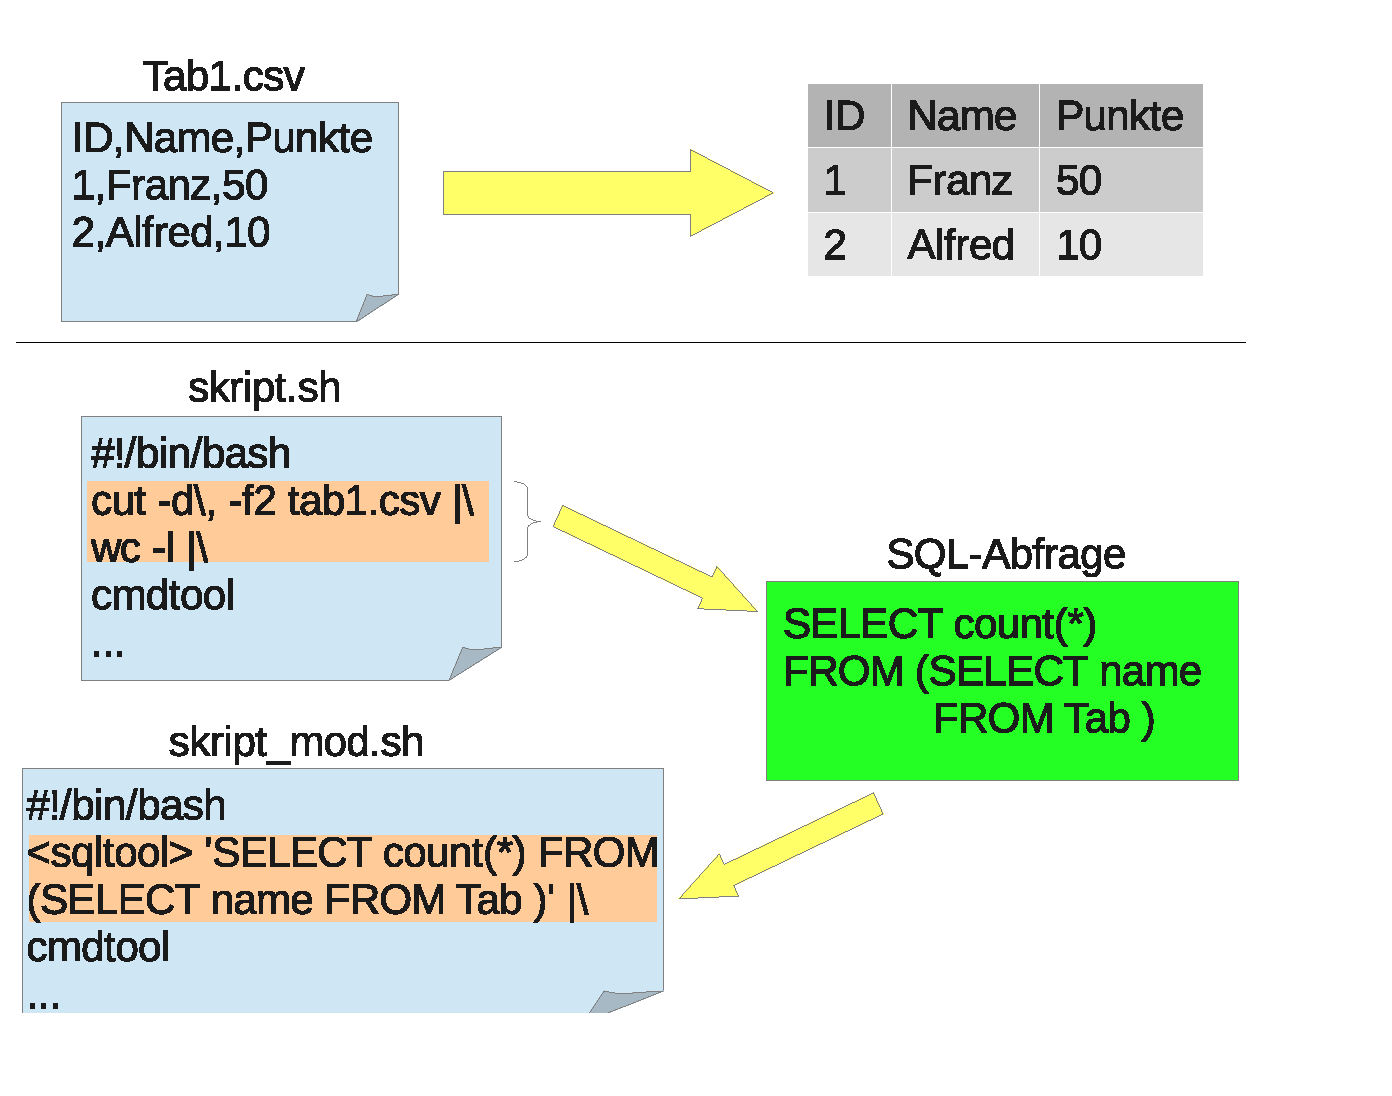
\includegraphics[scale=.5]{idee}
\caption{Grundidee: Daten werden vorab in eine Datenbank geladen, anschließend werden die Skripte übersetzt}
\label{fig:idee}
\end{figure}
Jetzt wird das Beste aus beiden Welten kombiniert - Bash-Skripte mit SQL-Abfragen. Soweit wie möglich sollen alle Kommandos eines Skripts in eine äquivalente SQL-Anweisung übersetzt werden. Um dennoch die Funktionen eines Skripts nicht zu verlieren, soll es möglich sein, die Abfrage in das Skript mittels eines Kommandos einzubinden, das die Abfrage auf einer Datenbank ausführt (\textit{SQL inline}).
Dazu wird ein Übersetzer geschrieben, der Shell-Skripte einliest und sie komplett oder teilweise in SQL-Abfragen übersetzt (siehe Abb. \ref{fig:idee}). So können die Vorteile eines Datenbanksystems mit einer einfachen deklarativen Sprache (SQL), mit parallelisierter Anfrageverarbeitung und deren Geschwindigkeit ausgenutzt werden, die Speicherung der Daten erfolgt aber weiterhin in CSV-Dateien.\\

\section{Textbasierte Datenbanken}
%Das Jahr 1970 bedeutete einen Umbruch im Bereich der Datenbanken, Edgar F. Codd veröffentlichte sein Papier über das relationale Modell, der Grundlage aller relationaler Datenbanken. Es erlaubt, mehrere Relationen zu verbinden, ohne dass der Benutzer sich um die interne Repräsentation kümmern muss \cite{Codd70}.
%Dennoch dauerte es weitere neun Jahre bis Larry Ellison und Bob Miner den ersten Prototyp einer relationalen Datenbank mit ihrer Firma Software Development Laboratories auf den Markt brachten, bei IBM sogar zwei Jahre länger \cite{Henderson03}.
%Dennoch werden Datensätze gerne noch in textbasierten Datenbanken (engl.: flat file databases) wie CSV-Dateien wegen ihrer Einfachheit gespeichert.\\

\begin{figure}[htb]
\centering
\begin{tabular}{p{3,5cm}|p{7,5cm}}
\hline
Franz Winkler & Am Winkl 5, 80000 Musterstadt\\ \hline
Xaver Ziegler & Maurergasse 19, 80000 Musterstadt\\ \hline
\end{tabular}
\caption{Beispiel für textbasierte Datenbank}
\end{figure}

%Textbasierte Datenbanken gibt es schon immer, sobald eine Person ein Adressbuch von Kontakten mit Namen und Adressen pflegt, so ist das eine textbasierte Datenbank. Sobald ein Kontakt den Wohnsitz wechselt oder die Anzahl an Freunden wächst, muss die Datenbank aktualisert werden, ist sie geordnet, bedeutet das in manchen Fällen, die Daten komplett neuzuschreiben, ein unnötiger Aufwand.\\
%Mit diesem Problem konfrontiert hat der deutschstämmige US-Amerikaner Hermann Hollerith bereits 1884 das erste Datenformat erfunden, \cite[S.48]{Bioinf08}, abgeschaut von Schaffnern in Zügen, die die Fahrkarten an bestimmten Stellen gelocht haben um Wiederverwendung auszuschließen, hat er die Lochkarte entwickelt. Das System wurde 1890 erstmals bei einer Volkszählung eingesetzt, wobei die Lochkarten die Informationen über Geschlecht und Alter enthielten und elektrische Maschinen in 3,4 Sekunden eine Karte auslasen. Weitere Aufträge auf der ganzen Erde folgten, Hollerith gründete die Computing Tabulating Recording Company (CTR), aus der 1924 schließlich IBM hervorging \cite{Heise07}.\\

%\begin{figure}
%\centering
%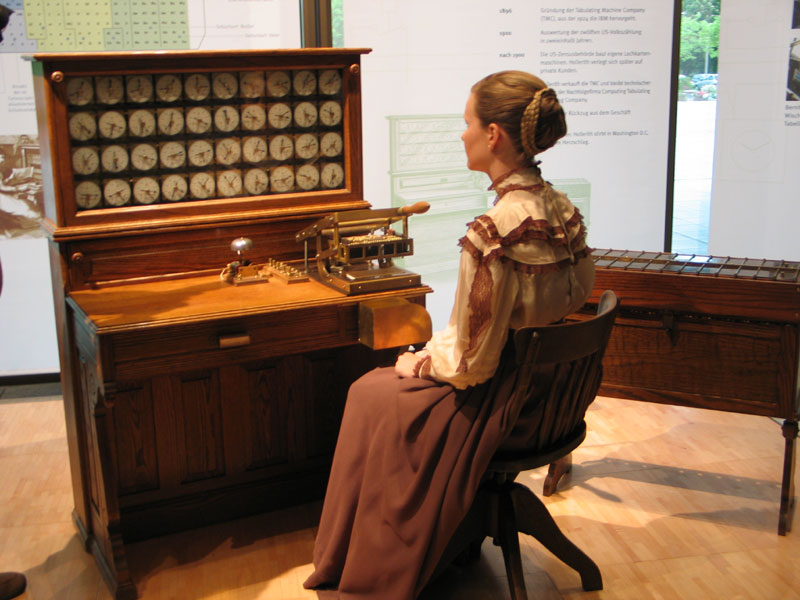
\includegraphics[scale=.2]{hollerith_machine.jpg}
%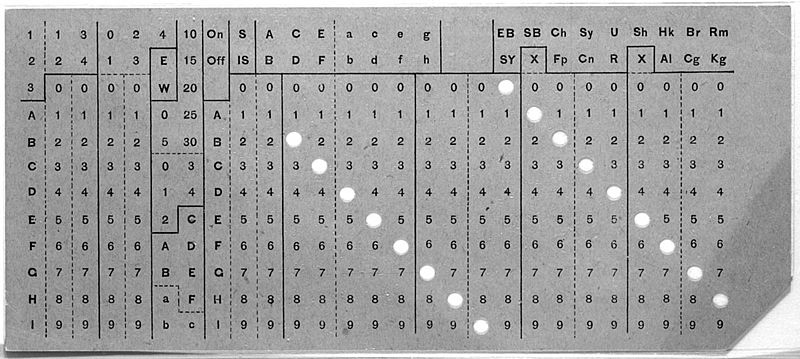
\includegraphics[scale=.7]{Hollerith_Punched_Card.jpg}
%\caption{Hollerith Maschine \cite{Heise07} mit Lochkarte [wikipedia.de]}
%\label{fig:hollerith}
%\end{figure}

%Textbasierte Datenbanken sind mittlerweile weit verbreitet, in Unix-Systemen (entwickelt Mitte der 1960-er Jahre) werden so Daten zum Beispiel zur Passwort- oder Gruppenverwaltung gespeichert. (siehe Abb. \ref{fig:passwd})
%Jeder Datensatz wird durch einen Zeilenvorschub mit Wagenrücklauf (engl.: carriage return und line feed, CRLF) abgeschlossen, einzelne Felder durch ein Trennzeichen (engl.: delimiter) separiert \cite{cql}. \\

%\begin{figure}
%\centering
%\fbox{\parbox{15cm}{
%root:x:0:0:root:/root:/bin/bash\\
%daemon:x:1:1:daemon:/usr/sbin:/bin/sh\\
%bin:x:2:2:bin:/bin:/bin/sh\\
%sys:x:3:3:sys:/dev:/bin/sh\\
%sync:x:4:65534:sync:/bin:/bin/sync
%}}
%\caption{Auszug aus /etc/passwd eines Unix-Systems mit Trennzeichen ':'}
%\label{fig:passwd}
%\end{figure}

Ein Beispiel für textbasierte Datenbanken sind CSV-Dateien (Comma-Separated Values) manchmal auch DSV-Dateien (Delimiter-Separated Values) genannt, also durch Komma oder anderes Trennzeichen separierte Tabellen. Erstmals zwischen 1968 und 1972 erwähnt als Teil der Fortran Spezifikation für listenorientierte Ein- und Ausgabe (Common Format and MIME Type for Comma-Separated Values (CSV) Files) \cite[S. 17]{IBM_Fortran}, haben sich CSV-Dateien zum Standard im Datenaustausch entwickelt.\\

Inzwischen existiert sogar eine Richtlinie für CSV-Dateien, herausgegeben von der Internet Engineering Task Force in der RFC\ 4180. Nach dieser Richtlinie soll jeder Datensatz einer CSV-Datei durch einen Zeilenvorschub mit Wagenrücklauf (engl., carriage return und line feed, CRLF) abgeschlossen und einzelne Felder durch ein Trennzeichen (engl.,\ delimiter) separiert sein \cite{RFC}.\\

Da die Richtlinie sich an DOS-Systemen (mit CRLF, '\textbackslash r\textbackslash n') orientiert, verwenden andere Systeme einen einfachen Zeilenvorschub (LF, '\textbackslash n'). Für gewöhnlich bestehen CSV-Dateien aus einem systemabhängigem Record Delimiter (zum Trennen von Datensätzen) und einem variablen Field Delimiter (Spaltentrennzeichen wie Komma) und orientieren sich an folgendem Schema:
\begin{itemize}
\item jeder Datensatz ist in einer Zeile gespeichert, beendet durch einen Record Delimiter
\item der letzte Datensatz benötigt keinen Record Delimiter
\item die erste Zeile kann eine Kopfzeile (engl., header) sein und muss für jede Spalte einen String als Bezeichner enthalten
\item die Felder sind durch einen Field Delimiter getrennt, nach der letzten Spalte muss kein Field Delimiter folgen; Leerzeichen sind Teil eines Feldes
\item jedes Feld kann in Anführungszeichen (doppelte Hochkommata, engl., double quoted fields) stehen
\item ein Feld, das Field Delimiter oder Record Delimiter enthält, muss in Anführungszeichen eingeschlossen sein
\item Anführungszeichen als Inhalt eines Feldes in doppelten Hochkommata (double quoted fields) werden escaped (durch eine Fluchtsequenz, z.B. '\textbackslash ')
\end{itemize}

Die Vorteile solcher Datenbanken liegen in ihrer Einfachheit, sie speichern alle Informationen, es werden keine weiteren Informationen benötigt, Import und Export von Informationen ist leicht, da außer einem Field bzw. Record Delimiter keine Konventionen einzuhalten sind.\\

Die Nutzung textbasierter Datenbanken bei Abfragen birgt aber Nachteile, so lassen sich die Daten speichern und verschicken, ein Ändern einzelner Datensätze erweist sich als schwierig, ohne die komplette Datei zu überschreiben. Da das Format nur wenigen Beschränkungen unterliegt, enthält in manchen Fällen die erste Zeile die Feldbezeichner, in anderen bereits den ersten Inhalt.
Aber das gravierendere Problem liegt in der Anzahl der Datensätze, jeder Datensatz muss zeilenweise ausgelesen werden, da auch keine Konventionen befolgt werden, ist auch nicht von einer Sortierung auzugehen. Analysen oder Datenänderungen sind auf diesem Format schwieriger und kostenaufwändiger als auf anderen, z.B. binär gespeicherten Daten.

\section{Vorgehen}
Im Nachfolgenden werden zuerst grundlegende Befehle erklärt, wie sie in Skripten zur Analyse von Textdateien vorkommen und auf bereits existierende Ansätze verwiesen, wie Daten in Textdateien bewältigt werden. Abschließend führt die Arbeit in die Welt der Parser und zeigt einen Ansatz auf, wie die Skripte übersetzt werden.
